\documentclass[pdflatex,sn-mathphys-num]{sn-jnl}% Math and Physical Sciences Numbered Reference Style

\usepackage{graphicx}%
\usepackage{multirow}%
\usepackage{amsmath,amssymb,amsfonts}%
\usepackage{amsthm}%
\usepackage{mathrsfs}%
\usepackage[title]{appendix}%
\usepackage{xcolor}%
\usepackage{textcomp}%
\usepackage{manyfoot}%
\usepackage{booktabs}%
\usepackage{algorithm}%
\usepackage{algorithmicx}%
\usepackage{algpseudocode}%
\usepackage{listings}%
\usepackage{rotating}
\usepackage{float}

\begin{document}

\title[Article Title]{Politics of emotions or propaganda?}

\author{\fnm{Timur} \sur{Rezepov 34177A}}

\affil{\orgdiv{Master's Degree Course in Data Science for Economics}}
\affil{\orgdiv{Natural Language Processing course, A.Y.  2024-2025}}
\affil{\orgdiv{Prof. Alfio Ferrara}}
\affil{\orgdiv{Dott. Sergio Picascia, Dott.ssa Elisabetta Rocchetti}}


\maketitle

\section{Introduction}\label{sec1}

This project explores how emotional language is used in political texts to influence perception and manipulate audience response. The data analyzed in the project is the transcription of US 2020 presidental debates available on Kaggle\footnote{US 2020 presidental debates: \\ https://www.kaggle.com/datasets/headsortails/us-election-2020-presidential-debates}. 

Emotion classification models based on pre-trained BERT architectures have been shown to outperform other approaches (Hsu and Ku, 2018\footnote{https://doi.org/10.18653/v1/W18-3505}). To obtain emotion annotations, the DistilBERT Classifier\footnote{https://keras.io/keras_hub/api/models/distil_bert/distil_bert_text_classifier/} was fine-tuned using some techniques and methods discussed in `GoEmotions: A Dataset of Fine-Grained Emotions`\footnote{https://arxiv.org/abs/2005.00547}. 


\section{Research question and methodology}\label{sec2}

Emotional language is a powerful tool in political speeches, used to persuade, mobilize, and connect with audiences on a deeper level. For example, words evoking fear or anger create a sense of urgency, while disapproval and guilt can create negative impressions of opponent's views.

This project aims to analyze the emotional language used by Donald Trump and Joe Biden in their speeches during the 2020 U.S. Presidential Election. Precisely, each candidate uses distinct communication strategies tailored to their target audiences, seeking to evoke specific emotional responses and strengthen their position.

The approach used comprises of building emotion profiles: the quantitative characteristic of how often different emotions(sentiments) used in the speech.
Specifically the analysis focuses on:
\begin{itemize}

	\item emotion flow throughout a single event;
	\item emotion profile during a specific debate event;
	\item comparison of emotional profiles across different debate events;
	\item emotion distribution by topic.
\end{itemize}

As part of the project, an emotion classification model was developed. The model is based on the pre-trained DistilBERT architecture, fine-tuned using the GoEmotions dataset. 

%%%%%%%%%%%%%%%%%%%%%%   SECTION 3   %%%%%%%%%%%%%%%%%%%%%%%%
\section{Experimental results}\label{sec3}
\subsection{Model training}

The GoEmotions dataset consists of 58,000 Reddit comments, each labeled with one or more of 27 emotions or marked as Neutral, making it a multi-label classification task.
Exploratory data analysis showed that the dataset is imbalanced. To address this, severely underrepresented classes were excluded, and only those emotions relevant to political discourse were retained—resulting in a set of 19 emotion classes.
\begin{figure}[h]
	\centering
	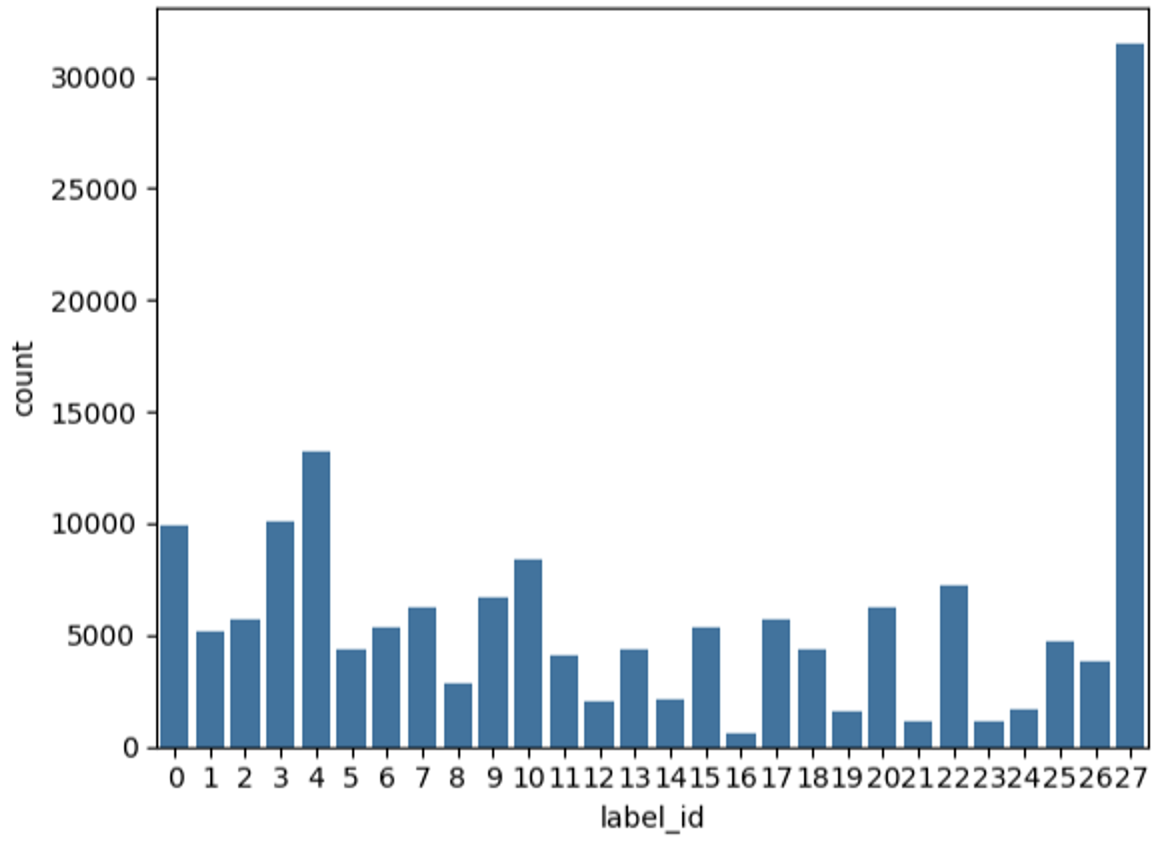
\includegraphics[width=10cm]{f1-label_distribution.png}
	\caption{Original class distribution in GoEmotions dataset}
\end{figure}

The model training parameters and performance metrics are summarised in Table 1.
The resulting accuracy can be considered reasonable given the complexity of the problem:
\begin{itemize}
	\item multi-classification problem with 19 classes; 
	\item imbalance of the dataset;
	\item emotional tone is subjective and each text can be classified differently by different experts.
\end{itemize}

The classification confusion matrix is shown in Figure 2.
\begin{table}[h]
	\caption{Model training parameters and performance metrics}\label{tab_2-1}%
	\begin{tabular}{@{}p{4cm}p{4cm}}
		\toprule
		Optimizer & Adam \\ 
		Learning Rate & 1e-5 \\ 
		Number of epochs & 2 \\
		Accuracy & 0.29\\ 
		\botrule
	\end{tabular}
\end{table}

\begin{figure}[h]
	\centering
	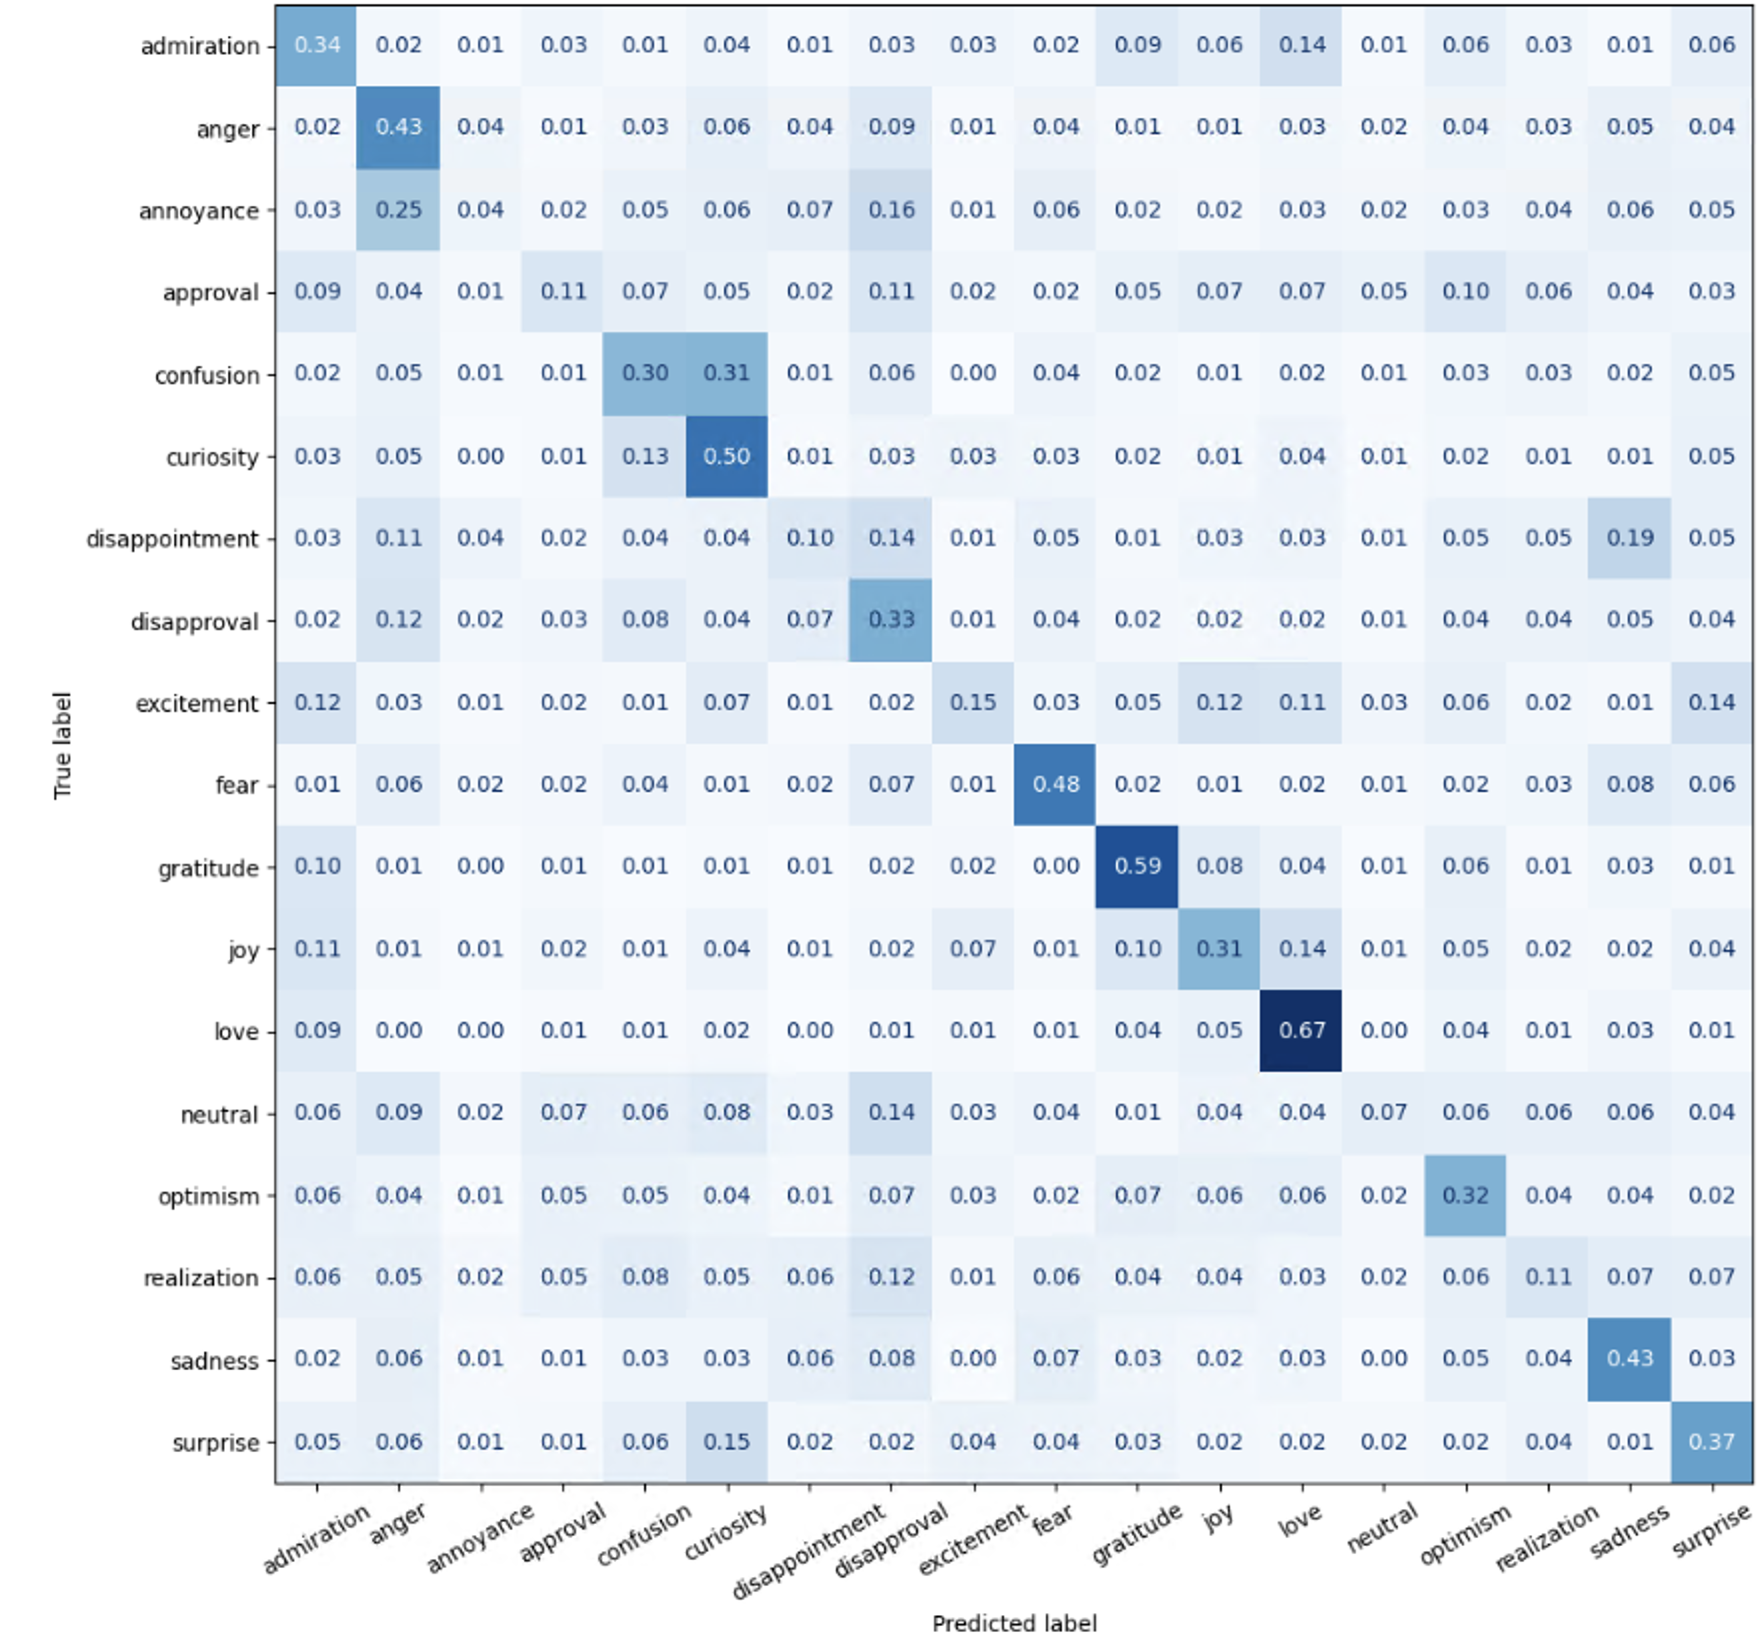
\includegraphics[width=12cm]{f2-confusion_matrix.png}
	\caption{Confusion matrix of the classifier}
\end{figure}

\subsection{Analysis of emotional language}
This article presents the key insights, while the more detailed analysis is available in the accompanying Jupyter Notebook within the repository.

\subsubsection{Emotion flow (single event)}

\begin{figure}[h]
	\centering
	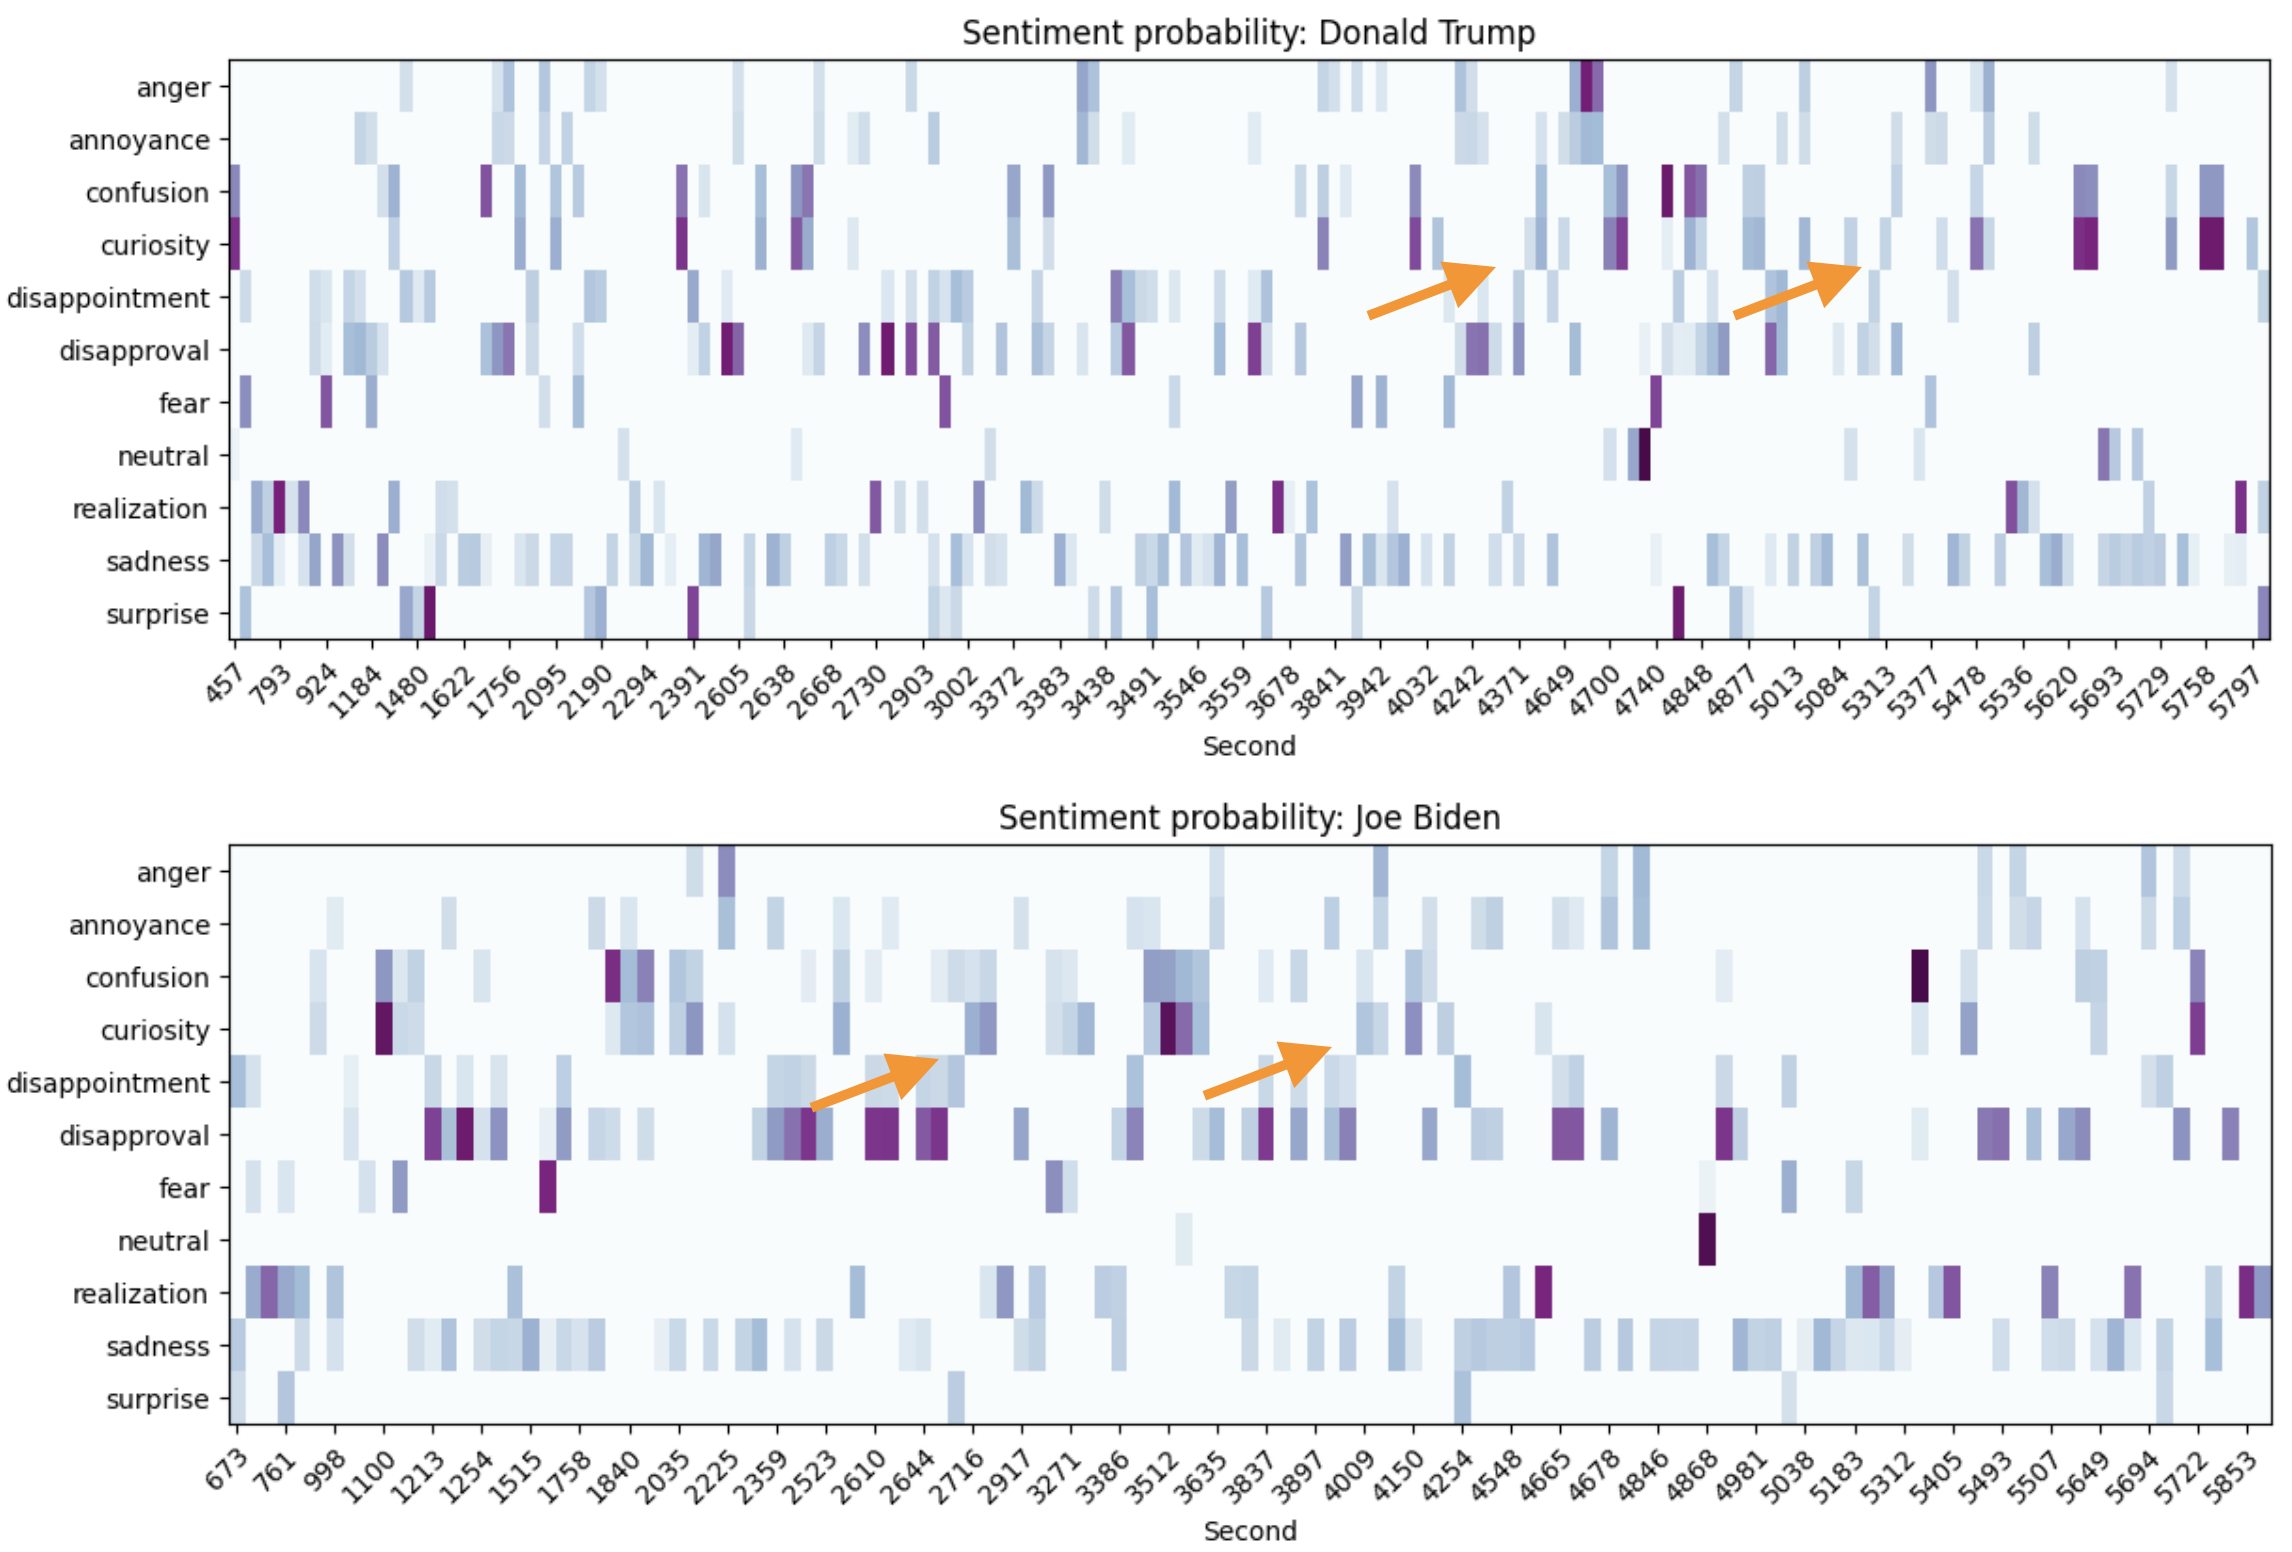
\includegraphics[width=13cm]{f3-emotion_flow.png}
	\caption{Emotion (sentiment)  flow}
\end{figure}

Fig. 3 demonstrates probabilities assigned by the classificator to speech during the 2nd presidental debates.
The emotional language of Donald Trump is more disperse and variable. Many emotions are short-lived and alternate.
Biden's language is more clustered: there are \texttt{series} of emotions. Also there are less \texttt{anger} spikes. This suggests the usage of more reflective, moral tone, while Trump prefers to stay unpredictable and provokable.

In the speech of both an interesting pattern can be noted: the consequetive chain of negative emotions \texttt{disapproval} - \texttt{disappointment} - \texttt{curiosity} - \texttt{confusion} - \texttt{annoyance} highlighted with orange arrows.

\subsubsection{Emotion profile (single event)}

Fig.4 demostrates emotion profile: share of each emotion expressed during the event.
Both speakers display a mostly similar profile. For instance, they use \texttt{approval} a lot to sound more constructive.
Trump's profile is more variable, he expresses \texttt{anger}, \texttt{admiration} and \texttt{surprise} suggesting a more expressive manner. The usage of \texttt{confusion} and \texttt{curiosity} is high: Trump uses questions to provoke the oponent, who, on the other hand, defended himself with \texttt{disapproval} and \texttt{annoyance}. 

\begin{figure}[h]
	\centering
	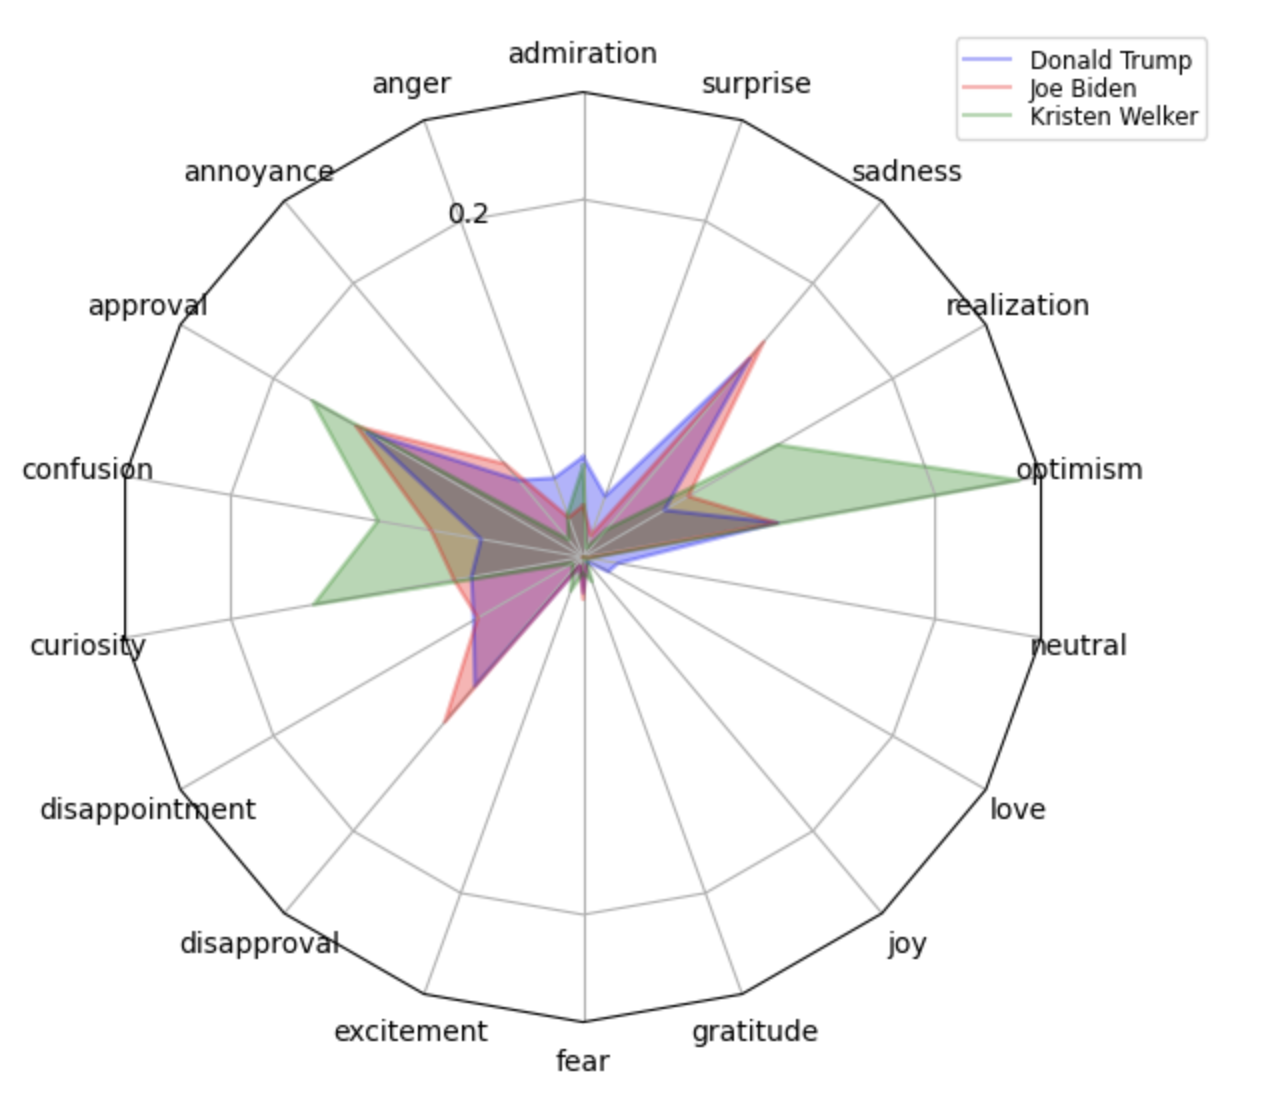
\includegraphics[width=14cm]{f4-emotion_profile.png}
	\caption{Emotion profile, 2nd presidental debate}
\end{figure}

\newpage
\subsubsection{Emotion profiles across debates}


Comparison of emotion profiles across two presidental debates is shown in Figure 5.
Both speakers demonstrate the same emotional shift: they express \texttt{optimism} and \texttt{sadness} more. \texttt{sadness} - due to the fact that they discussed COVID and it's impact, while \texttt{optimism} was used to balance it and form a more hopeful, foreward-looking message. Also they are less neutral, the seconds debate is less emotionally flat.

\begin{figure}[h]
	\centering
	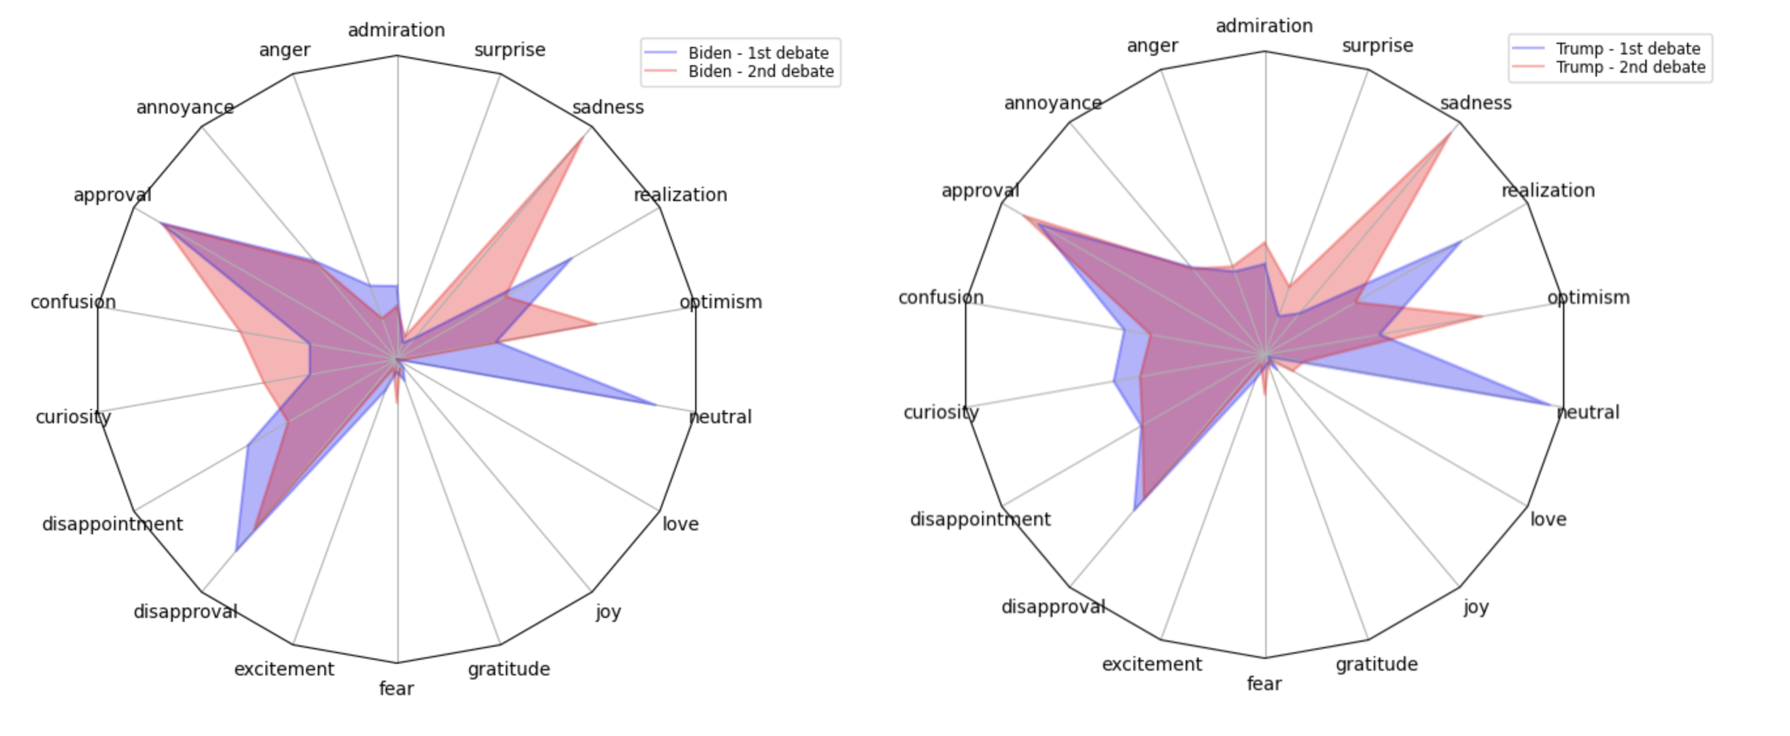
\includegraphics[width=14cm]{f5-debate_comparison.png}
	\caption{Debate comparison}
\end{figure}

\subsubsection{Topic modeling}

Topic modeling was used to analyze how emotional language varied across different topics. The topic markup was performed using BERTopic\footnote{https://maartengr.github.io/BERTopic/index.html}.

A clear example of emotional framing can be observed in the speakers' statements on the topic of Fracture and the Environment (Fig.6).

\begin{figure}[H]
	\centering
	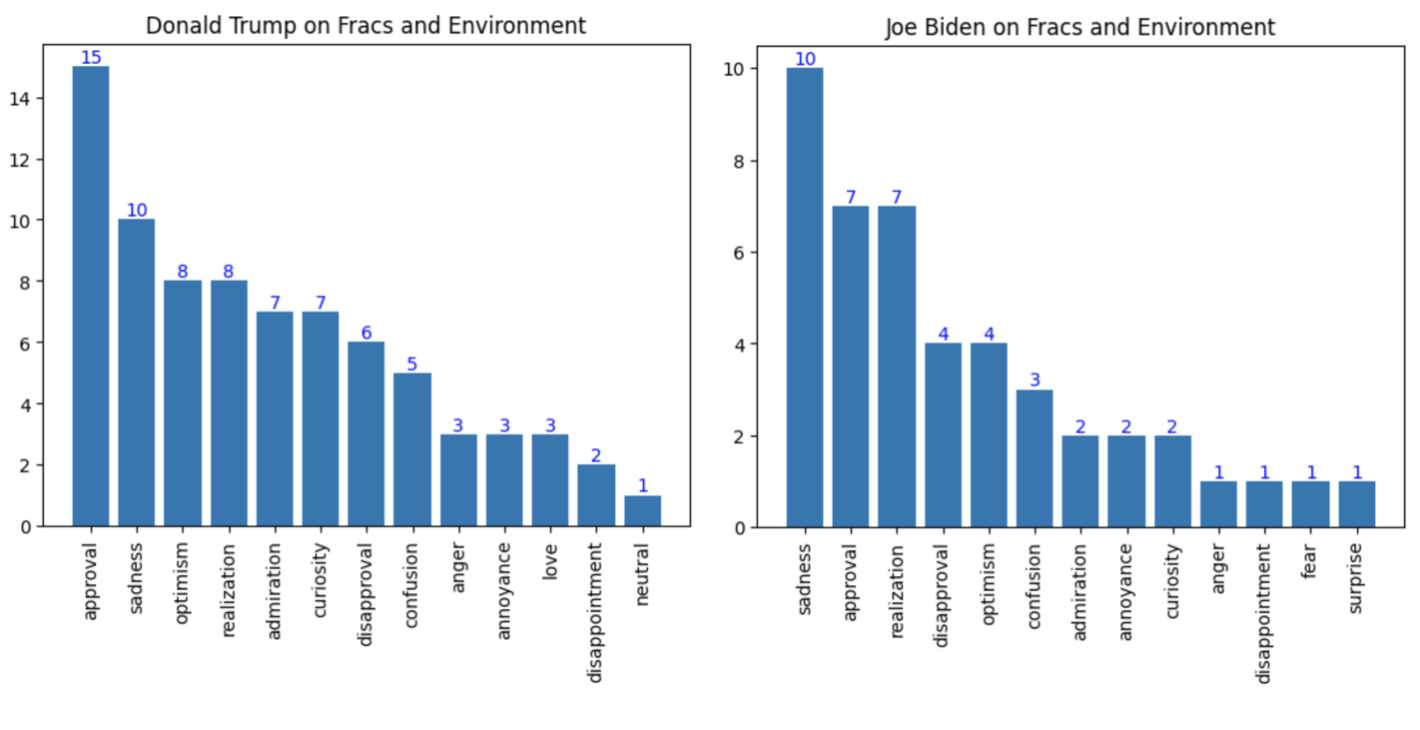
\includegraphics[width=14cm]{f6-fracture_and_environment.png}
	\caption{Emotion language used during discussions of Fracture and Environment}
\end{figure}

Biden expresses emotionally charged narrative: his speech has high levels of realization (personal awakening), sadness (for communities suffering cancer) and optimism (regulatory actions proposals). Biden uses personal memory (story about his childhood) to form emotional appeal and mobilize support.

Figure 7 presents the SHAP explainer’s output for one of Biden’s statements, which is rich in words and phrases evoking the emotion of \texttt{realization}.

\begin{figure}[H]
	\centering
	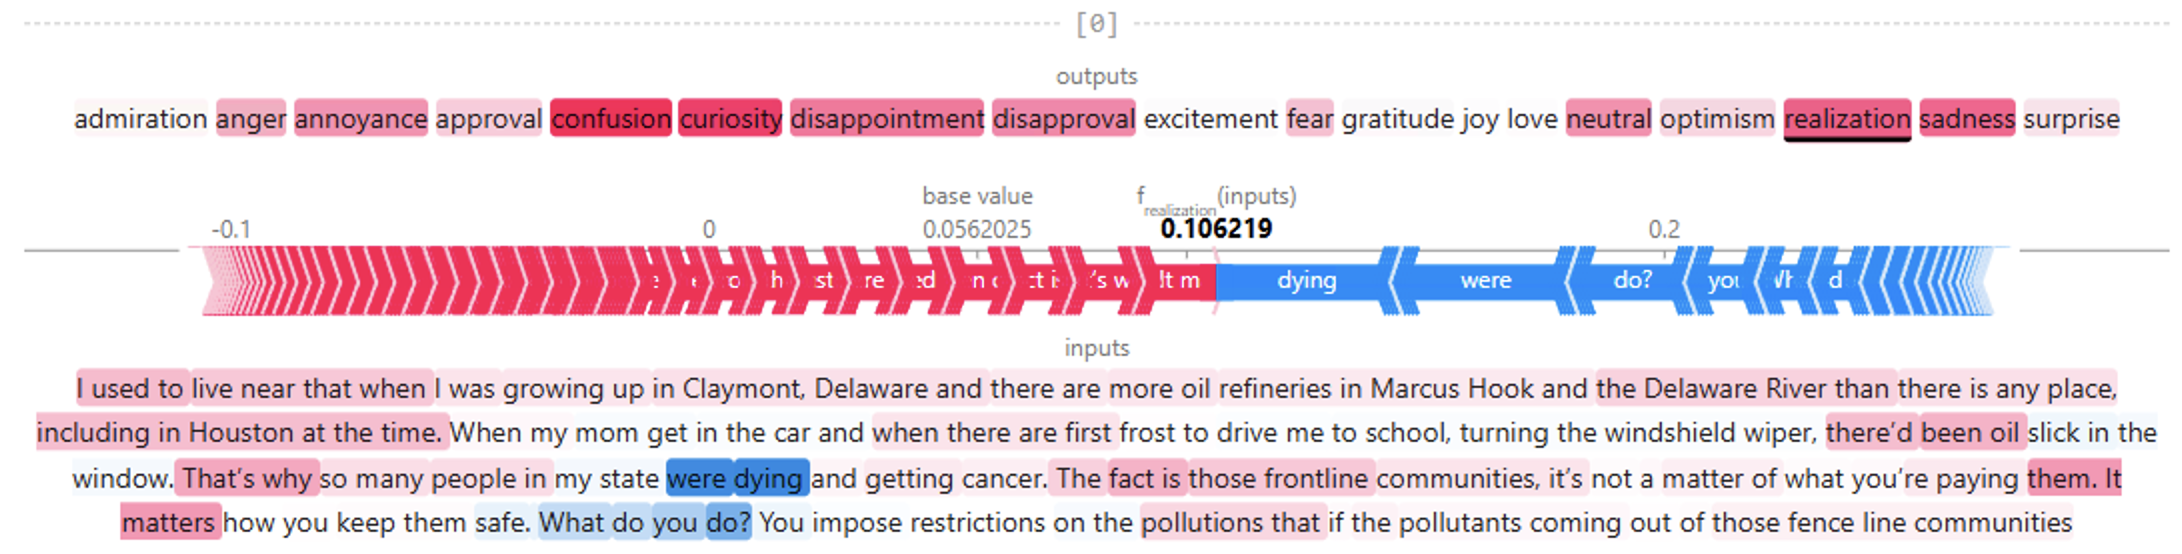
\includegraphics[width=12cm]{f7-explainer_realization.png}
	\caption{Emotion language used during discussions of Fracture and Environment}
\end{figure}

Trump's leading emotion is approval. He wants to justify his policie and evoke pride. His use of admiration and optimism suggests a strategic narrative of success and progress, often appealing to economic wellbeing.

Figure 8 shows the example of Trump using \texttt{admiration} in his speech.

\begin{figure}[H]
	\centering
	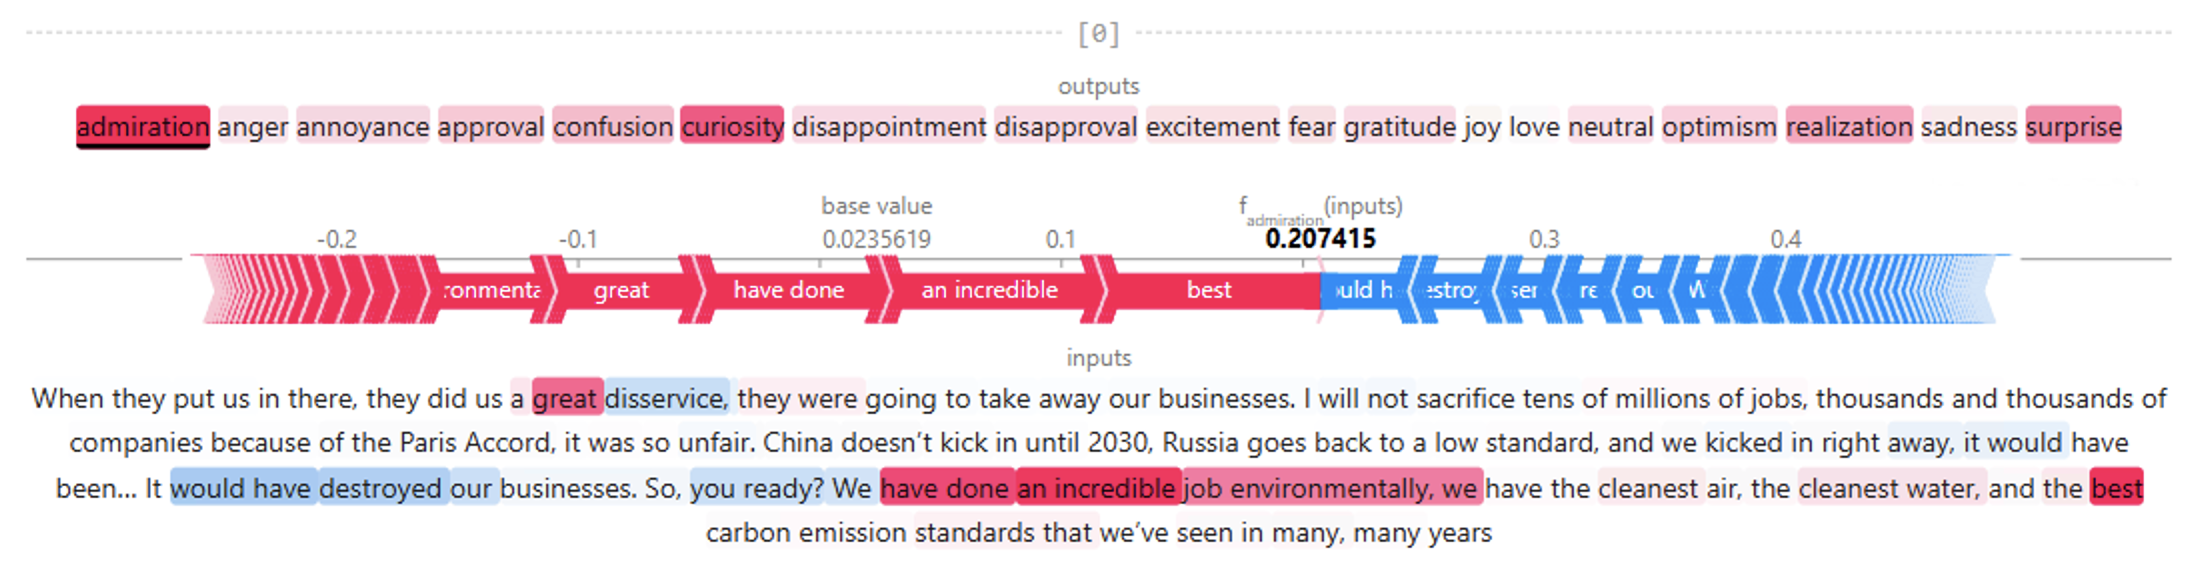
\includegraphics[width=12cm]{f8-explainer_admiration.png}
	\caption{Emotion language used during discussions of Fracture and Environment}
\end{figure}

\subsection{Conclusion}

The used model and methodology offer a foundation for emotion and sentiment analysis tasks.
The analysis demonstrated that emotional language is used broadly in political speeches. In the events studied, both Biden and Trump exhibited distinct emotional profiles: Biden’s language tended to be more empathetic and thoughtful, while Trump’s style appeared more provocative, expressive, and self-assured.

Future work could explore the following directions:

\begin{itemize}
	\item Improving classifier performance 
	\item Analyzing emotion distribution over longer timeframes (e.g., across multiple years)
	\item Constructing emotion network graphs or conducting turn-by-turn analyses to examine how one speaker’s statements influence the emotional tone of the other
	\item Investigating co-occurrence patterns among emotions
	\item Assessing the impact of emotional language on audience responses, such as through comment analysis or post-event surveys
\end{itemize}

\end{document}
